\chapter{Kalkulus Peubah Banyak}
Turunan peubah banyak lazim digunakan untuk mengoptimisasi jaringan saraf tiruan dengan menggunakan berbagai algoritma yang masuk dalam kategori penurunan gradien (\textit{gradient descent}), utamanya dengan menggunakan algoritma penurunan gradien stokastik (\textit{stochastic gradient descent}) (Gambar \ref{fig:fig4}). Sementara integral digunakan untuk memahami distribusi probabilitas kontinyu dalam teori probabilitas. Bagian ini hanya akan membahas kulit luar konsep - konsep di dalam kalkulus karena sifatnya sebagai pengantar semata.

\begin{figure}[H]
    \centering
    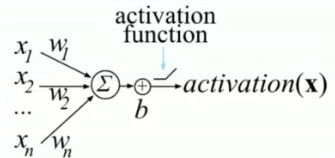
\includegraphics[width=0.5\textwidth]{gambar/gmb4.png}
    \caption{Optimasi algoritma jaringan saraf tiruan.}
    \label{fig:fig4}
\end{figure}

\section{Turunan}
Secara geometris turunan merupakan ukuran kemiringan dari suatu kurva atau yang sering disebut sebagai garis tangen. Kemiringan ini menyatakan ukuran perubahan kurva pada suatu titik tertentu. Sedangkan secara fisis, turunan merupakan laju perubahan suatu fungsi. Turunan satu dimensi dari fungsi $y=f(x)$ dinyatakan melalui notasi sebagai berikut(persamaan \ref{eqn:eqn19}):

\begin{dmath}\label{eqn:eqn19}
f'(x) = \frac{dy}{dx} = \frac{df(x)}{dx} = \frac{d}{dx}f(x)
\end{dmath}

Terdapat beberapa aturan di dalam penggunaan turunan di antaranya adalah sebagai berikut:
\subsection{Aturan turunan skalar}

\subsubsection{Konstanta}
Suatu konstanta karena sifatnya yang tetap, tidak akan pernah mengalami perubahan, maka berlaku:
\begin{equation}\label{eqn:eqn20}
    \frac{d}{dx} C = 0
\end{equation}
Contoh:
\begin{equation*}
    \frac{d}{dx}(128) = 0
\end{equation*}
\subsubsection{Aturan pangkat}
\begin{equation}\label{eqn:eqn21}
    \frac{d}{dx}x^{n} = nx^{n-1}
\end{equation}
Contoh:
\begin{equation*}
    \frac{d}{dx}x^{3} = 3x^{2}
\end{equation*}

\subsubsection{Perkalian}
\begin{equation}\label{eqn:eqn22}
    \frac{d}{dx}Cx^{n} = C\frac{d}{dx}x^{n} = Cx^{n-1}
\end{equation}
Contoh:
\begin{equation*}
    \frac{d}{dx}(4x^{3}) = 4\frac{d}{dx}x^{3} = 4(3)x^{2} = 12x^{2} 
\end{equation*}
\subsection{Aturan utama turunan}

\subsubsection{Aturan penjumlahan}
\begin{equation}\label{eqn:eqn23}
\frac{d}{dx}(f(x) + g(x)) = \frac{d}{dx} f(x) + \frac{d}{dx} g(x)    
\end{equation}
Contoh:
\begin{dmath*}
    \frac{d}{dx}(4x + 2x^{2}) = 4\frac{d}{dx}x^{2} + 2\frac{d}{dx}x^{2} = 4 + 4x
\end{dmath*}
\subsubsection{Aturan perkalian}
\begin{equation}\label{eqn:eqn24}
    \frac{d}{dx}(f(x).g(x)) = g(x)\frac{d}{dx}f(x) + f(x)\frac{d}{dx}g(x)
\end{equation}
Contoh:
\begin{dmath*}
    \frac{d}{dx}(x^{2}x) = x\frac{d}{dx}x^{2} + x^{2} \frac{d}{dx}x = x(2x) + x^{2} = 3x^{2}
\end{dmath*}

\sububsection{Aturan rantai}
Aturan ini penting untuk dipahami karena banyak digunakan di dalam analisis jaringan saraf tiruan.
\begin{equation}\label{eqn:eqn25}
    \frac{d}{{dx}}\left[ {f\left( u \right)} \right] = \frac{d}{{du}}\left[ {f\left( u \right)} \right]\frac{{du}}{{dx}}
\end{equation}
Contoh:
\begin{dmath*}
\frac{d}{dx}\sin{(x^{2})} = \cos{(x^2)}.2x = 2x\cos{(x^2)}
\end{dmath*}
\sububsection{Mengenal turunan parsial}
Turunan parsial digunakan untuk menyelesaikan permasalahan turunan yang melibatkan lebih dari satu peubah. Turunan parsial dua dimensi dinyatakan sebagai berikut(persamaan \ref{eqn:eqn26}):
\begin{equation}\label{eqn:eqn26}
    f'(x,y) = \nabla f(x,y) = \left[\frac{\partial f(x,y)}{\partial x}, \frac{\partial f(x,y)}{\partial y}\right]  
\end{equation}
Contoh:
\begin{eqnarray*}
f(x,y) = 3x^{2}y\\
\nabla f(x,y) = \left[\frac{\partial(3x^{2}y)}{\partial x}, \frac{\partial (3x^{2}y)}{\partial y} \right] = \left[3y(2x), 3x^{2}(1)\right] = \left[6xy, 3x^{2}\right]
\end{eqnarray*}

\section{Integral}
Konsep integral banyak digunakan untuk pemodelan distribusi probabilitas kontinyu yang digunakan dalam berbagai algoritma pemelajaran mesin. Metode integrasi umumnya digunakan untuk mencari luasan wilayah di bawah kurva (Gambar \ref{fig:fig5}). Proses integrasi merupakan kebalikan dari diferensiasi (turunan), maka integral sering dikenal sebagai anti-turunan. Formulasi umum integral ditunjukkan pada persamaan \ref{eqn:eqn27} berikut ini:
\begin{equation}\label{eqn:eqn27}
\int f'(x) dx = f(x) + C
\end{equation}
, dimana $C$ merupakan konstanta integrasi.

\begin{figure}[H]
    \centering
    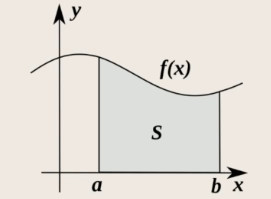
\includegraphics[width=0.5\textwidth]{gambar/gmb5.png}
    \caption{Ilustrasi integral untuk mencari luasan di bawah kurva.}
    \label{fig:fig5}
\end{figure}

\subsection{Jenis - jenis integral}
Terdapat dua jenis integral, yakni:
\subsubsection{Integral tak-tentu}
Integral tanpa batas yang diformulasikan sebagai berikut:
\begin{equation}\label{eqn:eqn28}
    \int f(x) dx
\end{equation}
\sububsection{Integral tentu}
Integral yang mempunyai batasan tertentu yang diformulasikan sebagai berikut:
\begin{equation}\label{eqn:eqn28}
    \int_{a}^{b} f(x) dx
\end{equation} 

\subsection{Aturan integral}
\subsubsection{Aturan pangkat}
\begin{equation}\label{eqn:eqn29}
    \int x^{n} dx = \frac{x^{n + 1}}{n + 1} + C
\end{equation}
Contoh:
\begin{equation*}
    \int x^{2} = \frac{x^3}{3} + C
\end{equation*}
\subsubsection{Aturan konstanta}
\begin{equation}\label{eqn:eqn30}
    \int k dx = kx + C
\end{equation}
Contoh:
\begin{equation*}
    \int 4 dx = 4x + C
\end{equation*}
\subsection{Penyelesaian integral tentu}
Berikut ini merupakan algoritma yang umum digunakan untuk menyelesaikan integral tentu:
\begin{dmath}\label{eqn:eqn31}
\int_{a}^{b} f'(x) dx = f(x)\big|_{a}^{b} = f(b) - f(a)
\end{dmath}
Contoh:
\begin{equation*}
\int_{0}^{2} 3x^{2} dx = 3 \int_{0}^{2} x^{2} dx = 3\left(\frac{x^3}{3}\right) \Big|_0^{2} = x^{3} \Big|_{0}^{2} = (2)^{3} - (0)^{3} = 8    
\end{equation*}
\section{Gradien}
Gradien umum digunakan untuk mengoptimasi algoritma jaringan saraf tiruan. Konsep gradien pada dasarnya berangkat dari turunan parsial yang seperti telah bersama kita ketahui dapat diorganisasikan ke dalam bentuk vektor(persamaan \ref{eqn:eqn32} merupakan contoh implementasi gradien pada dimensi tiga).

\begin{equation}\label{eqn:eqn32}
\nabla f(x,y) = \left[\frac{\partial f(x,y,z)}{\partial x}, \frac{\partial f(x,y,z)}{\partial y}, \frac{\partial f(x,y,z)}{\partial z}\right]
\end{equation} 

Seperti juga turunan, gradien merepresentasikan derajat kemiringan dari suatu fungsi. Gradien mengarah pada arah laju perubahan terbesar pada fungsi, dan besarannya menyatakan kemiringan pada arah tersebut. Dengan demikian gradien sangatlah cocok untuk digunakan untuk meminimalkan fungsi kerugian pada banyak algoritma pemelajaran mesin. Gradien tidak hanya terbatas pada dimensi tiga, kita dapat melakukan ekspansi pada dimensi - dimensi yang lebih besar seperti yang umum dilakukan ketika menerapkan algoritma pemelajaran mesin pada data raksasa.

Vektor gradien digunakan untuk menyusun turunan - turunan parsial dari suatu fungsi skalar. Ketika gradien diterapkan pada banyak fungsi, maka didefinisikan ke dalam bentuk matriks Jacobian. Formulasi matriks Jacobian untuk dua fungsi dengan dua buah peubah ditampilkan pada persamaan \ref{eqn:eqn33} sebagai berikut:

\begin{equation}\label{eqn:eqn33}
J = \begin{bmatrix}\nabla f(x,y) \\ \nabla g(x,y)\end{bmatrix} = \begin{bmatrix}\frac{\partial f(x,y)}{\partial x} & \frac{\partial f(x,y)}{\partial y} \\ \frac{\partial g(x,y)}{\partial x} & \frac{\partial g(x,y)}{\partial y} \end{bmatrix}
\end{equation} 

Formulasi umum untuk kasus dengan:
\begin{dmath*}
f(\mathbf{x}) = f(x_{1}, x_{2}, \cdots , x_{n}) 
\end{dmath*}
, adalah sebagai berikut (persamaan \ref{eqn:eqn34})

\begin{equation}\label{eqn:eqn34}
J = \begin{bmatrix} \nabla f_{1}(\mathbf{x})\\\nabla f_{2}(\mathbf{x})\\ \vdots \\ \nabla f_{m}(\mathbf{x})\end{bmatrix} = \begin{bmatrix} \frac{\partial f_{1}(\mathbf{x})}{\partial x_{1}} & \frac{\partial f_{1}(\mathbf{x})}{\partial x_{2}} & \cdots & \frac{\partial f_{1}(\mathbf{x})}{\partial x_{n}}\\ \frac{\partial f_{2}(\mathbf{x})}{\partial x_{1}} & \frac{\partial f_{2}(\mathbf{x})}{\partial x_{2}} & \cdots & \frac{\partial f_{2}(\mathbf{x})}{\partial x_{n}}\\ \cdots & \cdots & \cdots & \cdots\\\frac{\partial f_{m}(\mathbf{x})}{\partial x_{1}} & \frac{\partial f_{m}(\mathbf{x})}{\partial x_{2}} & \cdots & \frac{\partial f_{m}(\mathbf{x})}{\partial x_{n}}\end{bmatrix}
\end{equation}

\section{Laboratorium 3: Visualisasi gradien menggunakan matplotlib}
Pada bagian ini kita hendak melakukan visualisasi gradien untuk persamaan 2D.

Disini kita hendak berfokus pada pemahaman algoritma gradien, namun kita juga akan mempelajari beberapa konsep \textit{scripting} dengan menggunakan Python. Konsep - konsep tersebut antara lain adalah penggunaan \textit{meshgrid} yang sangat berguna untuk menampilkan informasi yang berhubungan dengan titik - titik berbeda di dalam suatu \textit{array}. Selain itu, kita juga akan mempelajari tentang pustaka matplotlib dengan menggunakan plot \textit{quiver} dan \textit{pcolor}.

\begin{pyin}
import sys
import numpy as np
import matplotlib
import matplotlib.pyplot as plt

print('Python: {}'.format(sys.version))
print('NumPy: {}'.format(np.__version__))
print('Matplotlib: {}'.format(matplotlib.__version__))
\end{pyin}

\begin{pyout}
Python: 3.8.3 (default, May 19 2020, 18:47:26) 
[GCC 7.3.0]
NumPy: 1.18.1
Matplotlib: 3.2.1
\end{pyout}

Sel di atas digunakan untuk mengimpor beberapa pustaka yang kita gunakan dalam sesi komputasi ini. 

Dengan menggunakan NumPy, kita membuat sebuah meshgrid untuk setiap titik $x$ dan $y$. \textit{Meshgrid} ini merupakan \textit{array} dua dimensi yang akan kita gunakan untuk visualisasi. Nilai $z$ pada setiap titik $x$ dan $y$ dihitung dengan menggunakan fungsi sebagai berikut:

\begin{pyin}
# menghasilkan meshgrid 2D
nx, ny = (100, 100)

x = np.linspace(0, 10, nx)
y = np.linspace(0, 10, ny)

xv, yv = np.meshgrid(x,y)

# mendefinisikan fungsi untuk plotting
def f(x,y):
    return x * (y**2)

# menghitung nilai z untuk setiap titik x,y
z = f(xv, yv)
\end{pyin}

Sekarang kita telah mempunyai \textit{meshgrid} dan telah menghitung $f(x,y)$ untuk seluruh titik di \textit{meshgrid}. Saatnya untuk memvisualisasikan hasilnya melalui \textit{colormap}.

\begin{pyin}
# Membuat colorplot untuk menampilkan data 
plt.figure(figsize=(14,12))
plt.pcolor(xv, yv, z)
plt.colorbar()
plt.show()
\end{pyin}

\begin{figure}[H]
    \centering
    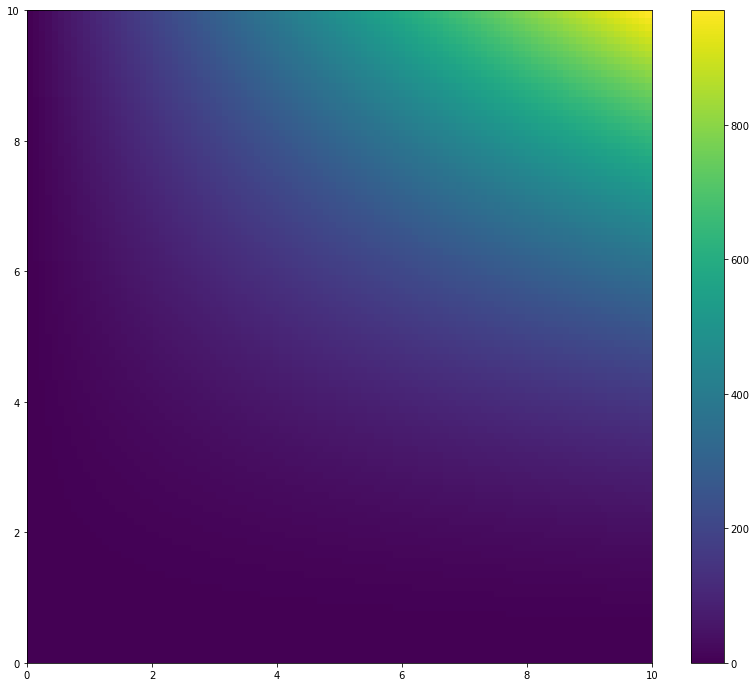
\includegraphics[width=0.5\textwidth]{gambar/gmb6.png}
    \caption{\textit{Colorplot} 2D dari fungsi $f(x,y)=xy^2$.}
    \label{fig:fig6}
\end{figure}

Sekarang saatnya kita menambahkan gradien ke dalam plot tersebut. Kita tidak akan menghitung gradien untuk setiap titik di dalam grafik ini, kita akan mendefinisikan \textit{meshgrid} baru dengan titik - titik yang lebih sedikit. Kita dapat memanfaatkan fungsi \verb|gradient()| di dalam pustaka NumPy untuk menghitung gradien pada setiap titik. Di sini kita harus berhati - hati karena prinsip kerja NumPy berbasis \textit{array}, maka luaran dari fungsi ini berupa baris, kolom bukan dalam format $x,y$.

\begin{pyin}
# membuat meshgrid 2D untuk gradien
nx, ny = (10, 10)
x = np.linspace(0, 10, nx)
y = np.linspace(0, 10, ny)
xg, yg = np.meshgrid(x,y)

# menghitung gradien untuk fungsi f(x,y)
# Catatan: NumPy menghasilkan luaran dalam format baris (y), kolom(x)
Gy, Gx = np.gradient(f(xg, yg))
\end{pyin}

Kemudian kita memvisualisasikan gradien menggunakan \textit{quiverplot} (Gambar \ref{fig:fig7}). Arah gradien direpresentasikan melalui anak panah, sedangkan besarannya direpresentasikan oleh panjang panah.

\begin{pyin}
# Memvisualisasikan gradien dengan colorplot
plt.figure(figsize=(14,12))
plt.pcolor(xv, yv, z)
plt.colorbar()
plt.quiver(xg, yg, Gx, Gy, scale = 1000, color = 'w')
plt.show()
\end{pyin}

\begin{figure}[H]
    \centering
    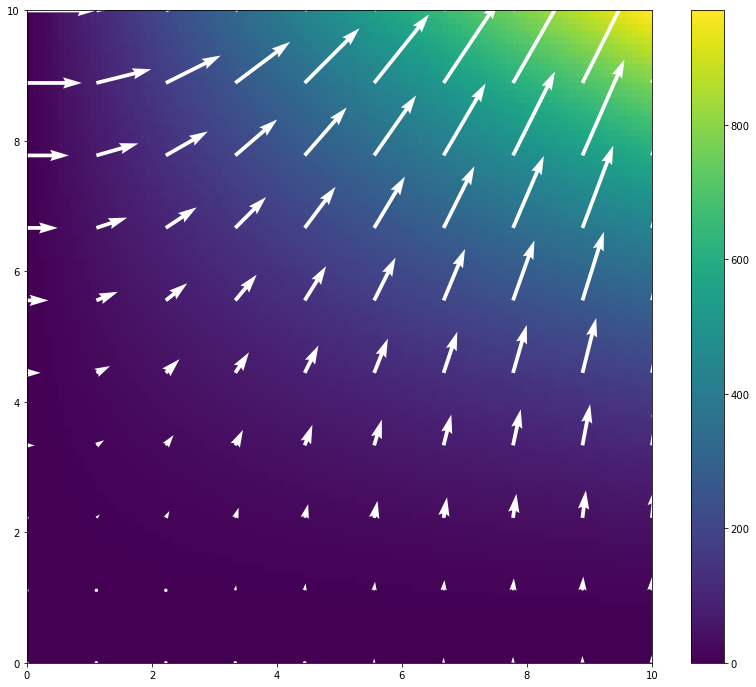
\includegraphics[width=0.5\textwidth]{gambar/gmb7.png}
    \caption{Gradien dari fungsi $f(x,y)=xy^2$.}
    \label{fig:fig7}
\end{figure}

\begin{pyin}
# Memvisualisasikan gradien dengan colorplot
plt.figure(figsize=(14,12))
plt.pcolor(xv, yv, z)
plt.colorbar()
plt.quiver(xg, yg, Gx, Gy, scale = 1000, color = 'w')
#plt.title('Gradient of f(x,y) = xy^2')
plt.show()
\end{pyin}

Plot di atas nampak sempurna. Anak - anak panah-nya nampak mengarah ke titik maksimum dan besarannya sesuai dengan kemiringan di setiap lokasi. Namun bagaimana kita bisa tahu kalau NumPy telah melakukan kalkulasi dengan benar? Untuk itu kita harus mencari turunan parsial melalui persamaan:

$$\nabla f(x,y) = \begin{bmatrix} \frac{d}{dx}f(x,y) && \frac{d}{dy}f(x,y) \end{bmatrix}$$

$$\nabla f(x,y) = \begin{bmatrix}y^2&&2xy\end{bmatrix}$$

Dengan mendefinisikan fungsi sebagai berikut:

\begin{pyin}
# menghitung gradien fungsi: f(x,y) = xy^2
def ddx(x,y):
    return y ** 2

def ddy(x,y):
    return (2 * y * x)

Gx = ddx(xg,yg)
Gy = ddy(xg,yg)
\end{pyin}

Kemudian kita memvisualisasikannya (Gambar \ref{fig:fig8}):

\begin{pyin}
# Plot
plt.figure(figsize=(14,12))
plt.pcolor(xv, yv, z)
plt.colorbar()
plt.quiver(xg, yg, Gx, Gy, scale = 1000, color = 'w')
plt.show()
\end{pyin}

\begin{figure}[H]
    \centering
    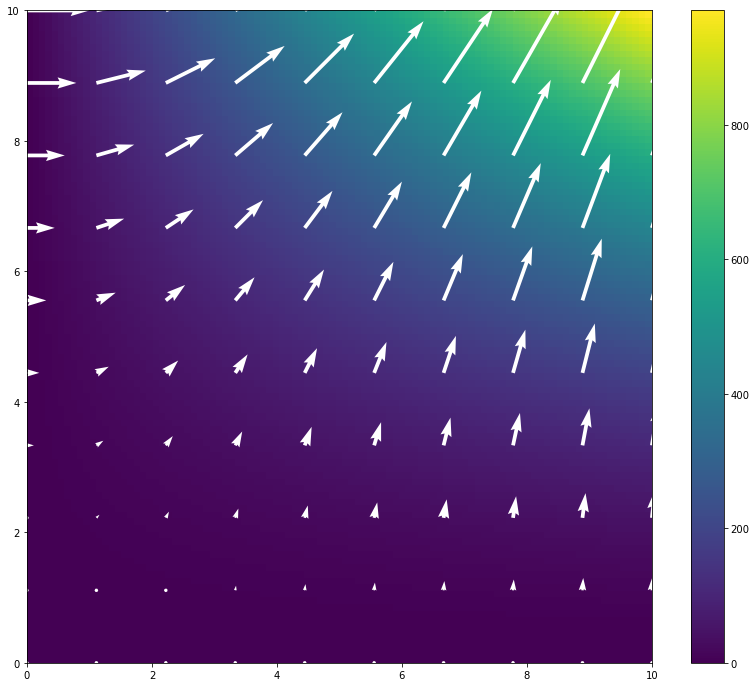
\includegraphics[width=0.5\textwidth]{gambar/gmb8.png}
    \caption{Visualisasi [$y^2$, $2xy$].}
    \label{fig:fig8}
\end{figure}

\section{Optimasi}
Pada bagian ini kita akan menggabungkan beberapa konsep yang telah kita pelajari pada bagian - bagian sebelumnya untuk memahami permasalahan optimasi pada fungsi konveks satu dimensi. Di dunia nyata tentunya kita akan disuguhkan oleh perkara optimasi yang melibatkan banyak dimensi, hanya karena buku ini hanya berupa pengantar matematis singkat, maka yang dibahas hanya pada perkara optimasi fungsi konveks berdimensi tunggal.  

Persamaan \ref{eqn:eqn35} menunjukkan formulasi umum dari optimasi fungsi konveks:

\begin{mini}|s|
{x}{f_{0}(x)}
{}{}
\addConstraint{f_{i}(x) \leq 0, i =\{i, \cdots, k\}}
\addConstraint{h_{j}(x) = 0, j = \{1,\cdots, k\}}
\label{eqn:eqn35}
\end{mini}
Berikut adalah beberapa terminologi yang wajib kita pahami:
\begin{itemize}
    \item $f_{0}(x)$: merupakan fungsi objektif yang hendak kita minimalkan (dalam kasus pemelajaran mesin merupakan fungsi kerugian).
    \item $x$: merupakan peubah objektif, umumnya di dalam algoritma jaringan saraf tiruan merupakan vektor masukan yang hendak kita \textit{update}.
    \item $f_{i}(x)$ dan $h_{j}(x)$ merupakan fungsi - fungsi kendala (\textit{constraint functions}) yang bentuknya dapat beragam.
\end{itemize}

Optimasi digunakan untuk mencari titik minimum global (Gambar \ref{fig:fig9}) dari suatu fungsi objektif yang mana harus memenuhi beberapa fungsi kendala.

\begin{figure}[H]
    \centering
    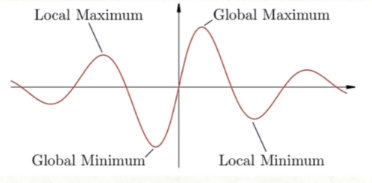
\includegraphics[width=0.7\textwidth]{gambar/gmb9.png}
    \caption{Visualisasi titik - titik kritis dari suatu fungsi objektif.}
    \label{fig:fig9}
\end{figure}

Jika fungsi objektif berupa fungsi konveks (cembung atau cekung), maka permasalahan optimasinya juga dikenal sebagai optimasi konveks. Pada fungsi konveks titik minimum yang hendak kita optimasi sudah pasti berupa titik minimum global.

Optimasi merupakan topik yang sangat penting di dalam analisis data karena hampir digunakan pada seluruh algoritma pemelajaran mesin, beberapa di antaranya adalah:
\begin{itemize}
    \item \textbf{Klasifikasi}:
    \begin{equation}
        \displaystyle{\minimize_{w} \sum_{i=1} \log(1 + \exp(-y_{i}x_{i}^{T}w)}
        \label{eqn:eqn36}
    \end{equation}
    \item \textbf{K-means}:
    \begin{equation}
        \displaystyle{\minimize_{\mu_{1}, \cdots, \mu_{k}}J(\mu) = \sum_{j=1}^{k}\sum_{i\in C_{j}}\lVert x_{i} - \mu_{j}\rVert^{2}}
        \label{eqn:eqn37}
    \end{equation}
    \item \textbf{Regresi logistik}:
    \begin{equation}
        \displaystyle{\minimize_{w} \lVert X_{w} - y \rVert^{2}}
        \label{eqn:eqn38}
    \end{equation}
\end{itemize}

Untuk lebih memahami persoalan optimasi ini kita akan mencoba menggunakan konsep turunan untuk mencari titik - titik kritis dari fungsi objektif $y = x^{2} + 3$ (Gambar \ref{fig:fig10}) dengan menggunakan turunan pertama dan kedua.
\begin{figure}[H]
    \centering
    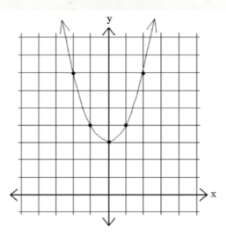
\includegraphics[width=0.5\textwidth]{gambar/gmb10.png}
    \caption{Fungsi  $y = x^{2} + 3$.}
    \label{fig:fig10}
\end{figure}

Yang pertama kali harus kita lakukan adalah mencari titik kritis dengan mengatur turunan pertama sama dengan nol:
\begin{equation*}
    y = x^{2} + 3
\end{equation*}
\begin{equation*}
    y' = 2x
\end{equation*}
\begin{equation*}
    0 = 2x
\end{equation*}
\begin{equation*}
    x = 0
\end{equation*}
Maka kita telah mengetahui titik kritis globalnya (karena fungsi ini merupakan fungsi konveks, maka seluruh titik kritisnya berlaku global). Untuk menguji apakah titik ini titik maksimum atau minimum, kita perlu melakukan penurunan kedua, yakni:
\begin{equation*}
    y'' = 2
\end{equation*}
Jika penurunan kedua bersifat positif, maka titik tersebut merupakan titik minimum, sedangkan jika bersifat negatif maka titik tersebut merupakan titik maksimum. Dalam kasus ini, maka titik minimum global dari fungsi $y = x^{3} + 3$ adalah $x = 0$.

Pencarian titik minimum global secara matematis tersebut umumnya tidak berlaku dalam konteks pemelajaran mesin. Karena volume data yang berjumlah sangat besar, maka diperlukan proses iteratif dengan menggunakan gradien. Jika gradien bernilai positif, maka kita menggeser ke arah lain hingga mendapatkan gradien yang bernilai negatif, dan hal ini dilakukan secara berulang hingga menemukan titik minimum yang dicari. Berikut ini contoh kasus yang mungkin dilakukan oleh algoritma pemelajaran mesin untuk mencari titik minimum:

\begin{enumerate}
    \item Tebakan pertama: $x=3$ merupakan titik minimum.
    \item Evaluasi $f(x)$:
    \begin{equation*}
        y = (3)^{2} + 3 = 12
    \end{equation*}
    \item Evaluasi nilai dari turunan:
    \begin{equation*}
        y' = 2(3) = 6
    \end{equation*}
    Ternyata gradien bernilai positif, maka kita harus mengubah arah tebakan.
    \item Tebakan kedua: $x = -1$ merupakan nilai minimum.
    \item Evaluasi $f(x)$:
        \begin{equation*}
           y = (-1)^{2} + 3 = 4
        \end{equation*}
    \item Evaluasi nilai dari turunan:
    \begin{equation*}
        y' = 2(-1) = -2
    \end{equation*}
    Ternyata tebakannya \textit{overshot}, maka kita ubah lagi arah tebakan.
    \item Begitu seterusnya hingga kita menemukan nilai $x = 0$ sebagai titik minimum.
\end{enumerate}

Proses ini dinamakan sebagai optimasi gradien stokastik. Pada algoritma jaringan saraf tiruan, jarak yang digunakan untuk mengubah arah tebakan umumnya tidak sebesar contoh di atas (dari 3 ke -2), melainkan sangatlah kecil (dari 3 ke 2,99 misalnya). Oleh karena volume data yang umumnya sangat besar, proses iterasi ini dapat berlangsung hingga ribuan, bahkan jutaan kali. 

Di dalam dunia nyata tentu tidak seluruh fungsi objektif yang hendak kita optimasi merupakan fungsi konveks, sehingga kita harus memperhitungkan juga titik - titik kritis yang bersifat lokal.